\chapter{Tinjauan Pustaka}
Pustaka yang digunakan dalam bab ini ialah acuan primer, diutamakan artikel jurnal dan paten yang relevan dengan bidang yang diteliti, terkini, dan asli (state of the art). Tinjauan pustaka memuat telaah singkat, jelas, dan sistematis tentang kerangka teoretis, kerangka pikir, temuan, postulat-postulat, prinsip, asumsi, dan hasil-hasil penelitian yang relevan yang melandasi masalah penelitian atau gagasan guna menggali pemahaman mengenai masalah penelitian dan pemecahan masalahnya. Oleh karena itu, dari tinjauan pustaka harus dapat diturunkan kerangka pikir, hipotesis penelitian, dan metode penelitian.

\section{Contoh Subbab}
Pariwisata merupakan sektor memberikan ciri khas. 

\subsection{Contoh Sub sub Bab}	    \textbf{Contoh Penulisan Persamaan} \\ 
 Persamaan kovarian antara \(Y_t\) dan \(Y_{t-k}\) pada semua lag \(k\) dijelaskan dalam Persamaan \ref{Persamaanobserver7}, sebagai berikut \cite{wei2006timeseries} :

\begin{equation} \label{Persamaanobserver7}
	\gamma_k = \text{Cov}(Y_t, Y_{t-k}) = \mathbb{E}[(Y_t-\mu_t)(Y_{t-k} - \mu_t)] 
\end{equation}
Keterangan:
\begin{align*}
	\rho_k & : \text{Fungsi autokorelasi} \\
	\gamma_k & : \text{kovarian antara } Y_t 
\end{align*}
\textbf{Contoh Penulisan Tabel} \\
\begin{table}[H]
	\centering
	\caption{Pola ACF dan PACF untuk komponen nonmusiman dan musiman}
	\label{tabel3}
	\begin{tabular}{lcccc}
		\toprule
		Model & \multicolumn{2}{c}{Nonseasonal} & \multicolumn{2}{c}{Seasonal} \\ \midrule
		& ACF & PACF & ACF & PACF \\
		\midrule
		AR & \textit{Dies down} & \textit{Cuts off} & \textit{Dies down} & \textit{Cuts off} \\
		&    & setelah \textit{lag} \(p\) &  &  setelah \textit{lag} \(P\) \\
		
		\bottomrule
	\end{tabular}
\end{table}
\textbf{Contoh Penulisan Gambar} \\
\begin{figure}[h!]
	\centering
	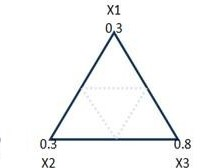
\includegraphics[width=8cm]{daerah1}
	\caption{Daerah rancangan awal kasus }
\end{figure}

	

		

	
	%\begin{figure}
	%	\begin{center}
		%		\includegraphics[scale=.5]{Gambar/observer.jpg} %masih kopi paste (perlu diganti)
		%	\end{center}
	%	\caption{Sistem Max-Plus dan Desain Observer} \label{observer}
	%\end{figure}
	
	

